In this section, we describe the environment setup that we use for developing our 3D shape retrieval system.
Python version 3.9 is the programming language in which the system is developed.
The reason for this choice is the rich assortment of Python libraries for 3D mesh manipulation, processing and
visualization - you can see our selection of them in \ref{tab:code_tools}, as well as our familiarity with the langauge.
The code for this project is available on the following  \href{https://github.com/cristi2019255/MultimediaRetrieval}{GitHub repository}.

\subsection{Dataset}
The dataset of 3D models we use for this project is a combination of the Princeton Shape
Benchmark \cite{Princeton} and the labeled PSB dataset \cite{PSB_dataset,PSB_paper}.
These datasets consist of a set of files in which the positions of vertices of the 3D shape are listed, along with a
set of indices describing the faces of the shape.
The shapes in this dataset are stored mostly in \verb!.off! and \verb!.obj! files.
However, we want to design a system that deals with all present kinds of file extensions for storing 3D objects.
Therefore, we convert \verb!.off! and \verb!.obj! files into \verb!.ply! files using a PyMeshLab \href{https://pymeshlab.readthedocs.io/en/latest/classes/meshset.html}{MeshSet class}.

In total, our final database has {} shapes.
\subsection{Database}
During the development of our retrieval system, one of the tasks we do is computing shape features and storing them
for all shapes in our dataset.
For this purpose and for ease of collaboration among the developers' team we chose to use a PostgreSQL database
hosted by Heroku (see the \href{https://github.com/cristi2019255/MultimediaRetrieval}{GitHub repository} for more
details).
This cloud database contains all relevant information of the shapes in the datasets that we use.
It contains for example the relative filepath for the 3D model, global information about the meshes such as the
amount of vertices and faces, and of course the features for the feature vector are stored there.
The data stored in this big cloud database will be inserted once after the preprocessing and feature extraction steps.
Once this is done, the querying for similar shapes can be done on the data that is stored there.

\subsection{Viewing 3D Models}
The visualization of the shapes is done using the PyVista library which has easy-to-use functions for loading and
displaying files, which can also be paired up with a custom theme.
For visualization, a list of files is passed to the function, and a new window is opened containing the faces and edges of the shape.
The window allows manipulation of the view of the visualization by zooming in, rotating, and moving the visualised
shape(s).
Additionally, the file name \& relative path are displayed above their respective figures.
An example of the visualization of two shapes from the dataset can be seen in Figure \ref{fig:initial}.

\begin{figure}[ht]
  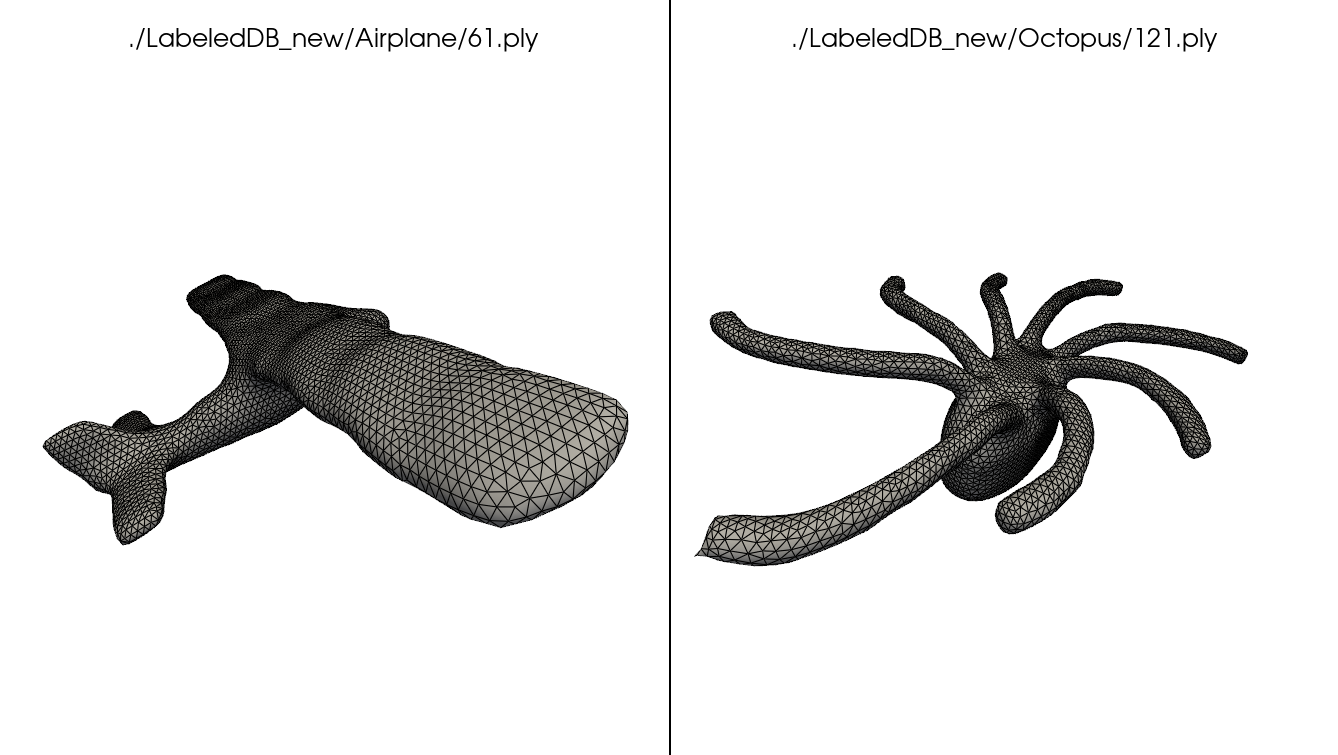
\includegraphics[width=\linewidth]{assets/visualisation/shapes_initial.png}
  \caption{Example of 3D mesh visualisation using PyVista. Models for an airplane and an octopus are visualised. The view of the models (size, rotation, position) can be modified.}
  \label{fig:initial}
\end{figure}
